\documentclass[border=2pt]{standalone}
\usepackage{fontspec}
\setmainfont{Liberation Serif}
\usepackage{tikz,graphicx,pgfplots}
\usetikzlibrary{arrows.meta,positioning,matrix,calc}
\pgfplotsset{compat=1.18}
\definecolor{forest}{HTML}{176044}
\definecolor{sage}{HTML}{EAF4EE}
\definecolor{rulec}{HTML}{CBD4CF}
\definecolor{ink}{HTML}{192723}
\definecolor{warm}{HTML}{F3ECE4}
\tikzset{all/.style={font=\fontsize{10.5pt}{12.5pt}\selectfont,text=ink},
box/.style={all,draw=rulec,fill=sage,rounded corners=2pt,align=center,inner sep=4pt,minimum height=0.9cm},
mutedbox/.style={box,fill=white},warmbox/.style={box,fill=warm},
flow/.style={-{Latex[length=2.4mm]},line width=.65pt,draw=forest}}
\begin{document}
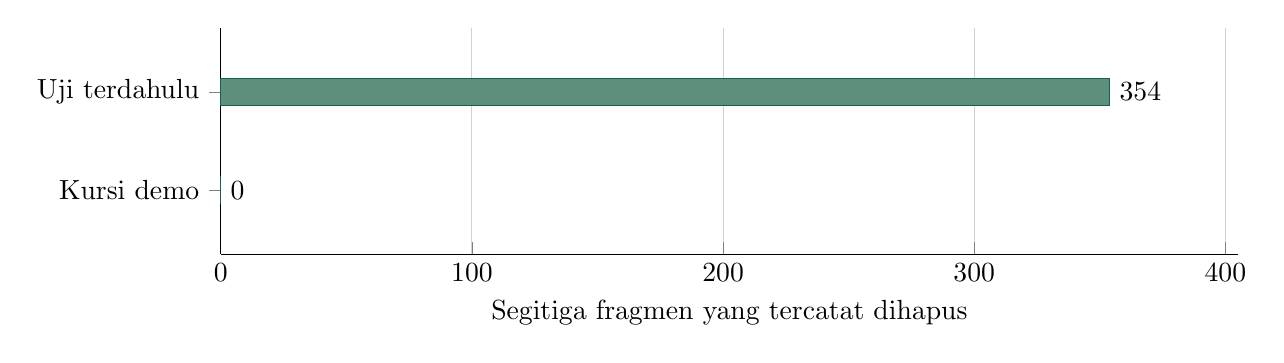
\begin{tikzpicture}[x=1cm,y=1cm]
\begin{axis}[xbar,xmin=0,xmax=405,xtick={0,100,200,300,400},
width=14.5cm,height=4.45cm,axis x line*=bottom,axis y line*=left,
symbolic y coords={Kursi demo,Uji terdahulu},ytick=data,
point meta=x,nodes near coords,clip=false,bar width=10pt,
xlabel={Segitiga fragmen yang tercatat dihapus},
tick label style={font=\fontsize{10pt}{12pt}\selectfont},
label style={font=\fontsize{10pt}{12pt}\selectfont},
nodes near coords style={font=\fontsize{10pt}{12pt}\selectfont},
xmajorgrids,grid style={rulec},enlarge y limits=.65]
\addplot[draw=forest,fill=forest!70] coordinates {(0,Kursi demo) (354,Uji terdahulu)};
\end{axis}
\end{tikzpicture}
\end{document}
